\documentclass[conference,spanish]{IEEEtran}

% ── Codificación y Lengua ──────────────────────────────────────────────────────
\usepackage[utf8]{inputenc}
\usepackage[T1]{fontenc}
\usepackage[spanish,es-noshorthands,es-tabla]{babel}

% ── Matemáticas ───────────────────────────────────────────────────────────────
\usepackage{amsmath, amssymb}

% ── Imágenes y diagramas ──────────────────────────────────────────────────────
\usepackage{graphicx}
\usepackage{float}
\usepackage{tikz}
\usetikzlibrary{positioning,arrows.meta}

% ── Tablas ────────────────────────────────────────────────────────────────────
\usepackage{booktabs}
\usepackage{array}

% ── Hipervínculos ─────────────────────────────────────────────────────────────
\usepackage[colorlinks=true, linkcolor=blue, urlcolor=blue, citecolor=blue]{hyperref}

% ── Otros ─────────────────────────────────────────────────────────────────────
\usepackage{microtype}
\usepackage{cite}

% ═══════════════════════════════════════════════════════════════════════════════
\begin{document}

\title{Predicción del Retraso en el Último Punto de Control de una Ruta de Bus Urbano en Cusco mediante Datos AVL y Aprendizaje Automático\\
\large Entregable 2 --- Aprendizaje Automático, PUCP 2026-2}

\author{
    \IEEEauthorblockN{
        Claudia Serpa,\;
        Nicoll Tone,\;
        Reynaldo Mamani,\;
        Jeremy Aldama
    }
    \IEEEauthorblockA{
        Facultad de Ciencias e Ingeniería,
        Pontificia Universidad Católica del Perú, Lima, Perú
    }
}

\maketitle

% ── Resumen ───────────────────────────────────────────────────────────────────
\begin{abstract}
Se predice, cuando un bus pasa por el punto de control 10 de 18, cuántos minutos llegará tarde o temprano al último punto de control de su vuelta. Se usa el registro de control de horarios del sistema de transporte inteligente de Cusco (\texttt{Times.csv}: 4\,707 vueltas de 45 buses con hora programada y real en 18 puntos de control, 6 de enero--1 de febrero de 2025). El retraso se recalcula en segundos y se aplican reglas de limpieza documentadas que conservan 4\,559 vueltas, 4\,004 de ellas con el último punto observado (la muestra para predecir). Además, se corrige la interpretación de 156 pasos anómalos: no son cruces de medianoche, como se supuso en la propuesta. Desde el punto 10 se compara tres líneas base (retraso cero, persistencia y media histórica por hora) con Ridge, Random Forest y HistGradientBoosting, cuyos hiperparámetros se ajustan con validación cruzada \textit{forward-chaining} por días; la prueba (27 de enero--1 de febrero) se evalúa una sola vez. HistGradientBoosting obtiene el menor error: MAE de 2,77 min (IC 95\,\% por día: 2,29--3,44) frente a 4,32 min de la persistencia, $R^2=0{,}76$ (0,62--0,83) y un 49\,\% de predicciones con error de 2 min o menos. Tiene menor MAE que las líneas base y que Ridge en los 6 días de prueba, y que Random Forest en 5 de 6 días (diferencia de 0,20 min, IC 0,02--0,37). También supera, en los 6 días, a una línea base más fuerte añadida tras la revisión: la media por hora y tipo de día (MAE 3,34 min). Desde P10, la estimación de $R^2$ queda por debajo de la meta de 0,80 fijada para este entregable, aunque con solo 6 días de prueba el IC no permite descartarla; en validación cruzada, la meta se alcanza desde P14. El error se concentra en los sábados, cuando el retraso crece de forma brusca en la segunda mitad de la ruta, y en un horario de tarde que aparece por primera vez en el periodo de prueba.
\end{abstract}

\begin{IEEEkeywords}
transporte público, AVL, predicción de retrasos, puntualidad, gradient boosting, validación temporal, Cusco
\end{IEEEkeywords}

% ═══════════════════════════════════════════════════════════════════════════════
\section{Introducción y Descripción del Problema}

En el transporte urbano de Cusco, la puntualidad respecto al horario programado es la principal medida de calidad que perciben los usuarios y que controlan los operadores. Las empresas ya registran, para cada vuelta, la hora programada y la hora real de paso por puntos de control, y monitorean la posición GPS de cada bus. Sin embargo, esa información se usa hoy para registrar o sancionar el retraso una vez ocurrido, no para anticiparlo.

Los datos muestran que el problema es real y crece a lo largo de la ruta. En los primeros puntos de control el retraso mediano es 0 o $-1$ min (los buses salen a tiempo o adelantados), pero desde el punto 14 la mediana sube a 1--3 min y el cuartil superior llega a 6--7 min. En el último punto, el 38\,\% de las vueltas llega más de 3 min tarde y el 17\,\% llega 2 min o más adelantada.

\textbf{Problema.} Dado el estado de una vuelta en un punto de control $k$ (retrasos observados hasta $k$, hora, día y vehículo; en la entrega final, también las velocidades GPS recientes), predecir el retraso en minutos en los puntos $k{+}1,\dots,18$. Formalmente, sea $d_{\ell,k}=t^{\mathrm{real}}_{\ell,k}-t^{\mathrm{prog}}_{\ell,k}$ el retraso de la vuelta $\ell$ en el punto $k$ (positivo si el bus va tarde). Se busca
\begin{equation}
\hat d_{\ell,j}=f_\theta\!\left(\mathbf x_{\ell,\le k},\, k,\, j\right),\qquad j>k,
\end{equation}
donde $\mathbf x_{\ell,\le k}$ contiene únicamente información disponible hasta el instante en que el bus pasa por $k$. La hora de llegada estimada es $\hat t^{\mathrm{real}}_{\ell,j}=t^{\mathrm{prog}}_{\ell,j}+\hat d_{\ell,j}$, la misma formulación residual sobre el horario que usan trabajos recientes de predicción de llegadas \cite{li2024arrivalnet,hu2022deepreta}. Esta tarea permite avisar al despachador o al usuario antes de que el retraso ocurra y ajustar la regulación de la flota (retener o adelantar buses).

\textbf{Por qué es un problema de aprendizaje automático.} El retraso depende de forma no lineal de la hora pico, del tramo, del conductor o vehículo y de la propagación del retraso previo. Una regla fija (``el retraso actual se mantiene'') es una línea base razonable, pero los resultados preliminares de la Sección~VI muestran que deja mucho error sin explicar.
\textbf{Organización.} La Sección~II presenta los objetivos; la III, los trabajos relacionados; la IV, el conjunto de datos y su preprocesamiento; la V, la metodología definitiva; la VI, los experimentos y resultados; la VII, la discusión y las limitaciones; la VIII, las conclusiones; y la IX, el entorno computacional para reproducir los experimentos.

% ═══════════════════════════════════════════════════════════════════════════════
\section{Objetivos}

\textbf{Objetivo general.} Desarrollar y comparar modelos de aprendizaje automático que predigan el retraso de un bus en el último punto de control de su vuelta, a partir de los datos de control de horarios de Cusco, con un error menor que el de las líneas base operativas.

\textbf{Objetivos específicos.}
\begin{enumerate}
    \item Limpiar \texttt{Times.csv} con reglas explícitas y cuantificadas, y caracterizar los problemas de calidad.
    \item Entrenar y comparar tres modelos de regresión (Ridge, Random Forest y HistGradientBoosting) contra tres líneas base, con validación temporal sin fuga de información.
    \item Reportar el error con intervalos de confianza y pruebas de significancia, y contrastarlo con dos metas fijadas antes de evaluar la prueba: superar a la mejor línea base en MAE y alcanzar $R^2\ge0{,}80$.
    \item Para la entrega final: evaluar todos los puntos de partida, incorporar variables del GPS (\texttt{Monitoring.csv}), la clasificación de puntualidad, el agrupamiento de perfiles de retraso y la demo interactiva.
\end{enumerate}
La meta de $R^2\ge0{,}80$ responde a la indicación del docente de fijar un umbral de desempeño del 80\,\%. Como el enunciado no especifica la métrica, se eligió $R^2$ porque es la proporción propia de la regresión y no depende de un umbral arbitrario de error. Tiene una limitación: depende de la varianza del objetivo en el conjunto evaluado, de modo que el mismo error absoluto da un $R^2$ distinto en días o subgrupos más o menos variables (Sección~\ref{sec:desglose}). Por eso la métrica principal sigue siendo el MAE en minutos, y el $R^2$ se usa solo para contrastar la meta.

% ═══════════════════════════════════════════════════════════════════════════════
\section{Trabajos Relacionados}

La predicción del tiempo de llegada y del retraso de buses es un tema amplio. La revisión de Reich et al.\ \cite{reich2019} concluye que ninguna familia de métodos domina en todos los contextos y que los resultados son poco comparables entre estudios; la de Kumar et al.\ \cite{kumar2025review} organiza los enfoques en ingenuos, basados en física y guiados por datos. Ello justifica comparar varios modelos bajo un mismo diseño experimental. La Tabla~\ref{tab:sota} resume los trabajos más cercanos.

\textbf{Primeros enfoques.} Chien et al.\ \cite{chien2002} y Jeong y Rilett \cite{jeong2004} usaron redes neuronales con datos AVL y superaron a los modelos históricos y de regresión. Yu et al.\ \cite{yu2006} aplicaron máquinas de vectores de soporte con variables de segmento, hora y tiempo de recorrido previo, y en paraderos con varias rutas SVM superó a redes neuronales, $k$-NN y regresión lineal \cite{yu2011}. Achar et al.\ \cite{achar2020} propusieron un filtro de Kalman espacial que aprende correlaciones entre tramos.

\textbf{Ensambles de árboles e interpretabilidad.} Martyanov et al.\ \cite{martyanov2026} es el trabajo más cercano a nuestra formulación: definen el retraso como la diferencia entre la llegada observada y la programada en cada parada, comparan Random Forest, XGBoost y CatBoost con validación cruzada temporal anidada y usan SHAP. Obtienen MAE $\approx$ 3,6 min y $R^2\approx$ 0,44, y encuentran que la hora del día y la posición en la ruta son las variables más influyentes porque el retraso se acumula a lo largo del recorrido.

\textbf{Aprendizaje profundo.} Petersen et al.\ \cite{petersen2019} emplearon una ConvLSTM multisalida sobre 1,2 millones de observaciones de una línea de Copenhague y redujeron el MAE de 3,23 min (media histórica) a 1,99 min. Boudabbous et al.\ \cite{boudabbous2026} predicen retrasos en toda la red de Montreal con LSTM, XGBoost y transformers bajo validación \textit{walk-forward}; una LSTM compacta (unos 31\,000 parámetros) ofrece el mejor compromiso entre precisión y eficiencia, y usan PCA para comprimir 1\,683 variables en 83 componentes conservando el 95\,\% de la varianza. Como en datos tabulares los modelos de árboles suelen igualar o superar a las redes profundas \cite{grinsztajn2022}, y nuestro conjunto tiene del orden de 4\,000 vueltas, se espera que el MLP y la LSTM no superen necesariamente a los ensambles. Por esa razón, y por el alcance de este entregable, no se incluyen en la comparación (Sección~\ref{sec:cambios}).

\textbf{Otros medios y escala industrial.} En servicios de movilidad, DeeprETA de Uber \cite{hu2022deepreta} predice el residuo entre la estimación del motor de rutas y la llegada observada, y el sistema Wide-Deep-Recurrent de DiDi \cite{wang2018wdr} corrige estimaciones base con un modelo aprendido. Ambos respaldan modelar la desviación respecto a una referencia (aquí, el horario) en vez de la llegada absoluta.

\textbf{Enfoques no supervisados.} Degeler et al.\ \cite{degeler2021} agrupan con $k$-means estados de operación (normal, retrasado, apelotonamiento) a partir de AVL y eligen $k$ con el coeficiente de silueta. En Cusco, Rojas-Bustamante et al.\ \cite{rojas2023} usaron aprendizaje no supervisado sobre trazas GPS de transporte público para perfilar la accesibilidad a servicios.

\textbf{Antecedentes en Perú.} Un trabajo con datos de Cusco \cite{cusco2024} aplica LSTM y ConvLSTM a 1,6 millones de registros GPS de buses y reporta un MAE de 19,55 s, pero predice tiempos de viaje, no el retraso respecto al horario. En Lima, Traverso et al.\ \cite{traverso2025} entrenaron Random Forest con registros de horarios del Corredor Metropolitano y reportan $R^2=0{,}9998$; valores tan altos, junto con una partición 70/30 sin descripción temporal, motivan cautela y subrayan la necesidad de una evaluación que evite la fuga de información \cite{kaufman2012}.

\textbf{Evaluación y umbrales.} En series temporales, la validación cruzada aleatoria puede inflar el desempeño \cite{bergmeir2012}; por ello se usa partición cronológica. En puntualidad de buses, una convención muy extendida considera a tiempo una llegada con hasta 1 min de adelanto y 5 min de retraso \cite{tcrp2003}; si en la entrega final se definen clases de puntualidad, sus umbrales se contrastarán con esa convención.

\textbf{Brecha que se aborda.} No se encontraron trabajos que predigan el retraso en puntos de control de rutas de Cusco, una ciudad con topografía y operación (puntos con horario fijo y sanciones por adelanto) distintas a las estudiadas. Este entregable usa solo el registro de control de horarios; la combinación con las velocidades GPS de la misma vuelta queda para la entrega final.

\begin{table*}[t]
\centering
\caption{Resumen de trabajos relacionados}
\label{tab:sota}
\footnotesize
\begin{tabular}{@{}p{3.4cm}p{4.3cm}p{4.0cm}p{4.9cm}@{}}
\toprule
\textbf{Trabajo} & \textbf{Datos} & \textbf{Modelos} & \textbf{Resultado clave}\\
\midrule
Yu \textit{et al.} 2006, 2011 \cite{yu2006,yu2011} & AVL; paraderos con varias rutas & SVM, ANN, $k$-NN, regresión lineal & SVM obtiene los mejores resultados\\
Achar \textit{et al.} 2020 \cite{achar2020} & GPS de buses, tráfico heterogéneo & Filtro de Kalman espacial & Captura correlaciones espacio-temporales por tramo\\
Petersen \textit{et al.} 2019 \cite{petersen2019} & Línea de Copenhague; 1,2 M obs. & ConvLSTM, LSTM, media histórica & MAE 1,99 min frente a 3,23 min (media histórica)\\
Martyanov \textit{et al.} 2026 \cite{martyanov2026} & AVL de Varsovia (retraso por parada) & RF, XGBoost, CatBoost + SHAP & MAE $\approx$ 3,6 min; RMSE $\approx$ 5,4 min; $R^2\approx$ 0,44\\
Boudabbous \textit{et al.} 2026 \cite{boudabbous2026} & Red de Montreal; seis meses & LSTM, XGBoost, xLSTM, transformers; PCA & LSTM compacta: mejor compromiso precisión--eficiencia\\
Degeler \textit{et al.} 2021 \cite{degeler2021} & AVL, apelotonamiento & $k$-means (silueta) & Estados: normal, retrasado, apelotonado\\
Trabajo en Cusco \cite{cusco2024} & 1,6 M registros GPS, Cusco & LSTM, ConvLSTM & MAE 19,55 s (tiempo de viaje)\\
Traverso \textit{et al.} 2025 \cite{traverso2025} & Corredor Metropolitano, Lima & Random Forest & $R^2=0{,}9998$ (requiere cautela)\\
Hu \textit{et al.} 2022 \cite{hu2022deepreta} & ETA global de Uber & Transformer lineal residual & En producción; modela el residuo de la ETA base\\
\bottomrule
\end{tabular}
\end{table*}

% ═══════════════════════════════════════════════════════════════════════════════
\section{Descripción del Conjunto de Datos}

Los dos archivos describen una sola ruta circular de 18 puntos de control, operada por 45 buses, y se pueden unir por vehículo, fecha y vuelta. Al cruzar la hora real de cada punto de control con el GPS más cercano ($\pm$60~s) se emparejó el 99,2\,\% de los pasos, y en el 99,1\,\% la vuelta coincide en ambos archivos. La Tabla~\ref{tab:datasets} resume ambos archivos.

\begin{table}[h]
\centering
\caption{Resumen de los archivos de datos}
\label{tab:datasets}
\footnotesize
\begin{tabular}{@{}p{1.6cm}p{3.1cm}p{3.1cm}@{}}
\toprule
\textbf{Atributo} & \textbf{Times.csv} & \textbf{Monitoring.csv}\\
\midrule
Registro & 1 vuelta de un bus (18 puntos) & 1 posición GPS\\
Cantidad & 4\,707 vueltas (84\,726 pasos) & 1\,630\,431\\
Periodo & 6 ene--1 feb 2025 (27 días) & 1 ene--1 feb 2025 (32 días)\\
Vehículos & 45 & 45\\
Variables clave & hora programada, hora real y diferencia por punto; vuelta & latitud, longitud, velocidad (km/h), rumbo, vuelta\\
Frecuencia & 4--6 vueltas por bus y día & cada 25~s (mediana); 90\,\% bajo 68~s\\
\bottomrule
\end{tabular}
\end{table}

\textbf{Estructura de \texttt{Times.csv}.} Las columnas \texttt{start\_time}, \texttt{end\_time} y \texttt{difference\_time} son arreglos de 18 valores; la primera hora programada coincide con la hora de partida. \texttt{difference\_time} es la parte entera de (hora real $-$ hora programada) en minutos: negativo implica adelanto y positivo, retraso. Como la parte entera descarta los segundos, el retraso se recalculó a partir de \texttt{start\_time} y \texttt{end\_time}. Existen cuatro plantillas de horario (147, 161, 168 y 170 min de vuelta programada); la de 161 min cubre el 65\,\% de las vueltas.

\textbf{Estructura de \texttt{Monitoring.csv}.} Cada registro contiene un identificador aleatorio, fecha, hora, vuelta, latitud, longitud, velocidad, rumbo e identificador del vehículo. En este entregable, el GPS se usa solo para ubicar los puntos de control y dibujar la ruta (Fig.~\ref{fig:ruta}, heredada de la propuesta y generada con \texttt{scripts/geo.py} y \texttt{scripts/more.py}); no se usa como variable predictora.

\textbf{Ubicación de los puntos de control.} Las coordenadas de los 18 puntos no se proporcionan: cada punto se ubicó con la mediana de las posiciones GPS en su hora real de paso. La ruta reconstruida sale del extremo este (P1), recorre la vía principal hacia el oeste hasta P10 y regresa al este (Fig.~\ref{fig:ruta}).

\begin{figure}[t]
\centering
\IfFileExists{ruta.png}{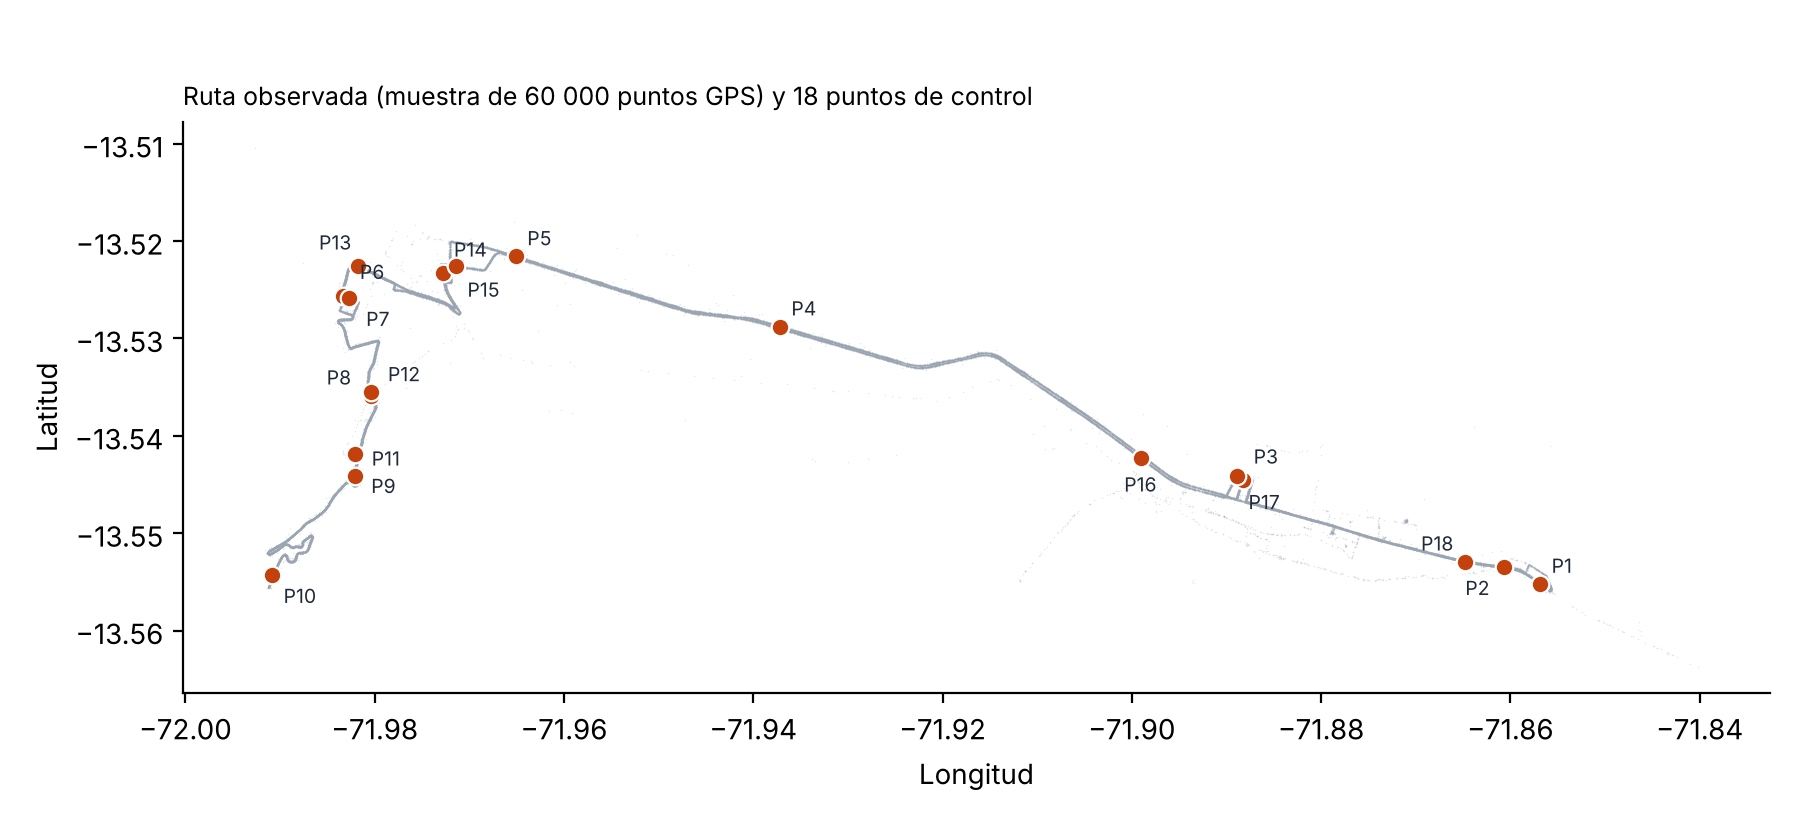
\includegraphics[width=\columnwidth]{ruta.png}}{\fbox{\parbox{0.9\columnwidth}{\centering\footnotesize [Insertar \texttt{ruta.png}: ruta reconstruida (muestra de 60\,000 puntos GPS) y los 18 puntos de control]}}}
\caption{Ruta reconstruida a partir de una muestra de 60\,000 puntos GPS (solo para visualización); cada punto de control se ubicó con la mediana de las posiciones GPS en su hora real de paso.}
\label{fig:ruta}
\end{figure}

\textbf{Calidad de datos.} Las reglas se fijaron antes de modelar y están implementadas en \texttt{src/01\_preprocesamiento.py}, que verifica con aserciones la estructura de los arreglos y de la salida. La Tabla~\ref{tab:calidad} cuantifica cada una. Tras la limpieza quedan 4\,559 vueltas (96,9\,\%), 4\,004 de ellas con el último punto observado; esta es la muestra para predecir el retraso en P18.

\begin{table}[h]
\centering
\caption{Problemas de calidad en \texttt{Times.csv} y tratamiento (sobre 4\,707 vueltas y 84\,726 pasos)}
\label{tab:calidad}
\footnotesize
\begin{tabular}{@{}p{2.3cm}p{2.5cm}p{2.9cm}@{}}
\toprule
\textbf{Problema} & \textbf{Magnitud} & \textbf{Tratamiento}\\
\midrule
Paso no registrado (``-'' y 00:00:00) & 7\,746 pasos (9,1\,\%) & NaN + indicador; el objetivo nunca se imputa\\
Horario programado no creciente & 148 vueltas (3,1\,\%) & Excluir la vuelta (arreglo corrupto)\\
Paso con hora incompatible con su vuelta ($|d|>60$ min) & 156 pasos (0,18\,\%) en 60 vueltas & Marcar el paso como NaN\\
Tramo con tiempo negativo & 30 vueltas antes de la regla anterior; 0 después & Excluir la vuelta (no se aplicó a ninguna)\\
Salto de retraso $>15$ min entre puntos consecutivos & 55 vueltas (1,2\,\%) & Conservar en entrenamiento y evaluación; solo se marca (puede ser un incidente real)\\
\bottomrule
\end{tabular}
\end{table}

\textbf{Corrección respecto al Entregable 1.} En el E1 los 156 pasos con $|d|>60$ min se atribuyeron a cruces de medianoche. Al revisarlos, ninguno está cerca de $\pm1\,440$ min, que es lo que produciría un cruce de medianoche. De los 156, 141 son negativos y 15 positivos, y se concentran en P11--P18 (46 en P18 y 30 en P16). El patrón dominante es claro: 122 de los 141 negativos tienen una hora de reloj entre las 4 y las 6 h, y 126 pertenecen a vueltas que salen entre las 16 y las 20 h. Por ejemplo, una vuelta que sale a las 18:52 registra en P18 la hora 05:45:20. Se contrastó si esas horas coinciden con pasos registrados de otras vueltas del mismo bus, el mismo día o el siguiente. Solo el 13\,\% queda a menos de 2 min de otro paso, frente al 33\,\% en pasos válidos desplazados al azar; por lo tanto, no se pudo verificar que sean pasos de otra vuelta. Una explicación compatible, que el GPS permitiría comprobar, es que el sistema cierra la vuelta inconclusa con la primera señal del día siguiente. Sea cual sea la causa, la hora es incompatible con la vuelta: el tratamiento no cambia (marcarlos como NaN), pero sí su justificación. Además, 93 pasos tienen $30<|d|\le60$ min y su clasificación es dudosa; la Sección~\ref{sec:umbral} muestra que bajar el umbral a 30 min no cambia los resultados.

\textbf{Otros hallazgos.} (i) La documentación del dataset describe \texttt{difference\_time} como el ``tiempo total del tramo''. Se verificó que en realidad es la parte entera (truncada, no redondeada) de (real $-$ programada) en el 100\,\% de los pasos observados. Usar el retraso con segundos mejora su resolución sin cambiar su significado. (ii) Hay 106 huecos en la numeración de vueltas, entre 3\,522 pares consecutivos del mismo bus y día. No es posible saber si esas vueltas no se hicieron o no se registraron; por eso el número de vuelta es poco fiable, y de hecho casi no aporta al modelo (Sección~\ref{sec:imp}). (iii) En P18, 229 de las 642 vueltas con plantilla de 147 min (36\,\%) llegan más de 10 min adelantadas; salen entre las 4 y las 6 h y el adelanto aparece desde P5--P6. Una hipótesis, no contrastada aquí, es que el tráfico de madrugada es menor que el que supone el horario. (iv) Cambio de horario en el periodo de prueba: la plantilla de 170 min (salidas de 16 a 20 h) aparece solo hasta el 24 de enero. Desde el 27 de enero, las salidas de esa franja usan una plantilla nueva de 168 min, que no existe en el desarrollo (234 vueltas de prueba). Se detectó al examinar el periodo de prueba después de la evaluación única, como parte del análisis del error, y no se modificó el modelo congelado. Su efecto se analiza en la Sección~\ref{sec:desglose}.

\textbf{Análisis exploratorio.} Para no guiar decisiones con la prueba, se hace solo sobre el desarrollo (3\,465 vueltas; 3\,082 con P18). La Fig.~\ref{fig:eda_punto} muestra que el retraso mediano oscila entre $-1{,}6$ y 1,6 min hasta P13, salta a 3,7 min en P14 y queda en 2,4 min en P18. La dispersión, en cambio, se abre desde P14: el p90 pasa de 7,7 min en P13 a 12,4 en P14. P17 es el punto con más pasos no registrados (27\,\%). La Fig.~\ref{fig:eda_p18} muestra que el retraso en P18 depende sobre todo de la hora de salida: es negativo de madrugada (plantilla de 147 min), y cercano a cero a mediodía. De 16 a 19 h, la mayoría de las salidas usa la plantilla de 170 min, con medianas de $-1$ a 9 min; las pocas que usan la de 161 min (8--27 vueltas por hora) llegan a medianas de 17--24 min. Por día, el sábado se separa claramente: mediana de 10,8 min frente a 1,1--2,5 min de los demás días.

\begin{figure}[t]
\centering
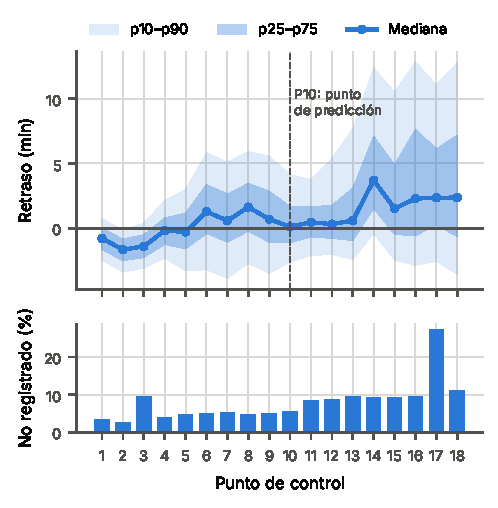
\includegraphics[width=\columnwidth]{figuras/eda_por_punto.pdf}
\caption{Desarrollo (6--26 ene): 3\,465 de las 4\,559 vueltas conservadas. Arriba: retraso por punto de control (mediana, rango intercuartílico y p10--p90). Abajo: porcentaje de pasos no registrados.}
\label{fig:eda_punto}
\end{figure}

\begin{figure*}[t]
\centering
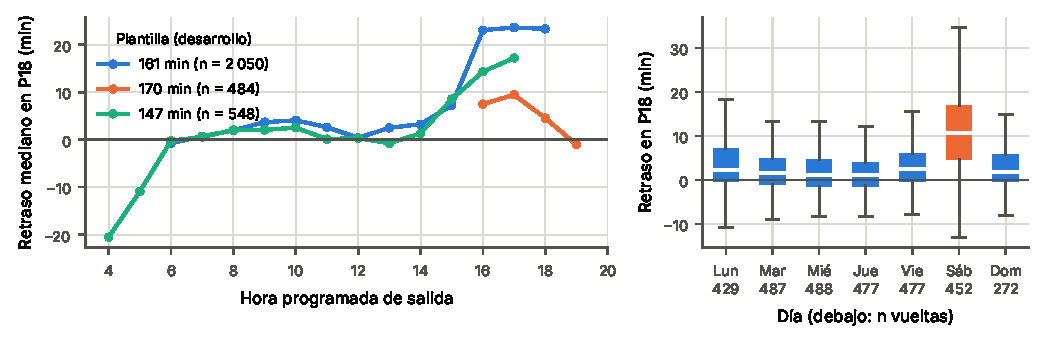
\includegraphics[width=\textwidth]{figuras/eda_p18.pdf}
\caption{Retraso en P18 en el desarrollo: 3\,082 de las 4\,004 vueltas con P18 observado. Izquierda: mediana por hora programada de salida y plantilla (se omiten horas con menos de 10 vueltas; la plantilla de 168 min no aparece en el desarrollo). Derecha: distribución por día de la semana, sin valores atípicos; el sábado se resalta.}
\label{fig:eda_p18}
\end{figure*}

% ═══════════════════════════════════════════════════════════════════════════════
\section{Metodología}

\subsection{Cambios respecto al Entregable 1}\label{sec:cambios}
Por indicación del docente, el alcance de este entregable se centró en que la regresión funcione bien y se midiera con rigor. Los cambios son:
\begin{itemize}
    \item \emph{Tarea:} la ecuación~(1) es multihorizonte, pero este entregable fija el objetivo en P18 (de ahí el cambio de título). El experimento principal es el experimento base del E1, que predice el retraso en P18 desde P10. Como análisis complementario, se mide el error según el punto de partida ($k=5,\dots,17$) solo con validación cruzada. La clasificación y el agrupamiento pasan a la entrega final.
    \item \emph{Datos:} solo \texttt{Times.csv}. Las variables GPS requieren unir 1,6 millones de registros por tramo, y ese archivo no forma parte del repositorio; se incorporarán en la entrega final.
    \item \emph{Modelos:} tres líneas base y tres modelos. Se retiran SVR, Lasso, el árbol individual, el MLP y la LSTM. Con 4\,004 vueltas y datos tabulares, se espera que los ensambles de árboles sean la referencia fuerte \cite{grinsztajn2022}. Comparar muchos modelos sobre solo 6 días de prueba produciría diferencias difíciles de distinguir del ruido.
    \item \emph{Métrica operativa:} se mantiene el porcentaje de predicciones con error $\le2$ min definido en el E1, y se añade la meta $R^2\ge0{,}80$ (Sección~II).
    \item \emph{Transparencia sobre la prueba:} los resultados preliminares del E1 ya se calcularon sobre el mismo periodo de prueba. Para no seguir usándolo, todas las decisiones de este entregable (limpieza, variables, hiperparámetros) se tomaron solo con validación cruzada dentro del periodo de desarrollo. El protocolo se congeló en un \textit{commit} antes de evaluar la prueba, y los modelos se evaluaron en la prueba una sola vez; el script registra la evaluación y se niega a repetirla. Después de esa evaluación sí se examinaron el periodo de prueba y las predicciones guardadas para analizar el error: desglose por día y por plantilla, descubrimiento de la plantilla nueva y la comparación estadística por día de la Sección~\ref{sec:comparacion}. Estos análisis son posteriores y descriptivos, y no modificaron ningún modelo.
\end{itemize}

\subsection{Variables}
Todas las variables están disponibles cuando el bus pasa por P10, es decir, son causales (20 en total):
\begin{itemize}
    \item \emph{Propagación:} retrasos $d_1,\dots,d_{10}$ (con NaN si el paso no se registró), último retraso observado, su variación respecto al anterior observado y número de pasos faltantes.
    \item \emph{Horario:} hora programada de salida (seno y coseno), plantilla (duración programada) y tiempo programado restante hasta P18.
    \item \emph{Calendario y operación:} día de la semana, número de vuelta del día y vehículo (45 vehículos, con 39--91 vueltas de desarrollo cada uno; mediana 70).
\end{itemize}
Se evaluó además el retraso final de la vuelta anterior del mismo bus, que tiene correlación 0,35 con el objetivo. Es causal, porque en ninguna vuelta la salida programada es anterior a la llegada real de la vuelta previa. Vale NaN si hay un hueco en la numeración. La regla, fijada antes de calcularla, era incluirla solo si bajaba el MAE de validación cruzada en al menos dos de los tres modelos. Con la configuración por defecto bajó en HistGradientBoosting (3,484 $\to$ 3,466 min), pero subió en Random Forest (3,566 $\to$ 3,585) y en Ridge (3,789 $\to$ 3,798). No se incluyó. En cualquier caso, la mejora en HistGB (0,02 min) es muy inferior a la desviación entre pliegues (0,9 min), así que la decisión no afecta las conclusiones.

\subsection{Modelos}
\begin{itemize}
    \item \emph{Líneas base:} retraso cero (horario perfecto); persistencia (el último retraso observado se mantiene hasta P18); media histórica del retraso en P18 por hora entera de salida (17 franjas, de 4 a 20 h), calculada solo con el entrenamiento de cada pliegue, con la media global para horas sin datos. Todas las franjas tienen al menos 30 vueltas de desarrollo, salvo una con 1.
    \item \emph{Ridge:} imputación por mediana con indicadores de faltante, estandarización y \textit{one-hot} del vehículo y del día.
    \item \emph{Random Forest} \cite{breiman2001}: imputación por mediana con indicadores; 300 árboles.
    \item \emph{HistGradientBoosting} (implementación de \textit{gradient boosting} con histogramas de scikit-learn, análoga a LightGBM \cite{ke2017}): maneja los NaN de forma nativa, con el vehículo y el día como variables categóricas.
\end{itemize}
Toda imputación, escalado y codificación está dentro de un \textit{pipeline} que se ajusta solo con los datos de entrenamiento de cada pliegue \cite{pedregosa2011,kaufman2012}.

\subsection{Diseño experimental}
\textbf{Partición.} Cada vuelta se asigna a un conjunto por su fecha de salida y nunca se divide. El desarrollo abarca del 6 al 26 de enero (21 días, 3\,082 vueltas) y la prueba, del 27 de enero al 1 de febrero (6 días de lunes a sábado, 922 vueltas).

\textbf{Validación cruzada \textit{forward-chaining} por días} (ventana de entrenamiento expansiva, también llamada \textit{walk-forward}). Dentro del desarrollo, el primer pliegue entrena con los primeros 11 días y valida con los 2 siguientes; cada pliegue posterior añade esos 2 días al entrenamiento y valida con los 2 siguientes. Son 5 pliegues, con 1\,655--2\,836 vueltas de entrenamiento y 225--331 de validación. Así nunca se valida con días anteriores a los de entrenamiento \cite{bergmeir2012}, y la selección de hiperparámetros usa 10 días de validación en vez de los 5 previstos en el E1.

\textbf{Ajuste de hiperparámetros.} Búsqueda aleatoria (\texttt{RandomizedSearchCV}) que minimiza el MAE medio de los 5 pliegues: 40 configuraciones para cada ensamble y 30 para Ridge. La Tabla~\ref{tab:hiper} muestra los espacios y los valores elegidos. Luego, cada modelo se reentrena con todo el desarrollo y se evalúa una vez en la prueba.

\begin{table}[h]
\centering
\caption{Hiperparámetros: espacio de búsqueda y valor elegido}
\label{tab:hiper}
\scriptsize
\begin{tabular}{@{}p{1.1cm}p{2.8cm}p{2.6cm}p{0.9cm}@{}}
\toprule
\textbf{Modelo} & \textbf{Parámetro} & \textbf{Espacio} & \textbf{Elegido}\\
\midrule
Ridge & $\alpha$ & log-uniforme $[10^{-3},10^{3}]$ & 1,22\\
\midrule
Random & \texttt{max\_depth} & \{None, 6, 10, 16\} & None\\
Forest & \texttt{min\_samples\_leaf} & \{1, 2, 5, 10, 20\} & 5\\
 & \texttt{max\_features} & \{0,3; 0,5; 0,8; 1,0\} & 0,8\\
\midrule
HistGB & \texttt{learning\_rate} & log-uniforme $[0{,}01;0{,}2]$ & 0,034\\
 & \texttt{max\_iter} & \{100, 200, 400, 800\} & 400\\
 & \texttt{max\_leaf\_nodes} & \{7, 15, 31, 63\} & 7\\
 & \texttt{min\_samples\_leaf} & \{5, 10, 20, 40\} & 40\\
 & \texttt{l2\_regularization} & log-uniforme $[10^{-3},10]$ & 0,0099\\
\bottomrule
\end{tabular}
\end{table}

\textbf{Estabilidad de la selección.} Las 5 mejores configuraciones de cada modelo difieren en menos de 0,02 min de MAE de validación cruzada: HistGB 3,375--3,393, Random Forest 3,533--3,566 y Ridge 3,790--3,800. Esa diferencia es muy inferior a la desviación entre pliegues (alrededor de 0,9 min en los ensambles). Por eso el valor exacto elegido no es crítico. Frente a la configuración por defecto, el ajuste baja el MAE de validación cruzada en 0,11 min en HistGB (3,48 $\to$ 3,38), en 0,03 min en Random Forest y nada en Ridge. Son ganancias pequeñas frente a la variabilidad entre pliegues: los modelos son robustos a sus hiperparámetros, y el ajuste no explica la ventaja de los ensambles. La lista completa está en \texttt{resultados/hiperparametros\_top5.csv}.

\subsection{Métricas y comparación estadística}
\begin{itemize}
    \item \emph{Principal:} MAE en minutos. \emph{Complementarias:} RMSE, $R^2$ y porcentaje de predicciones con error absoluto $\le2$ min (operativa, definida en el E1).
    \item \emph{Intervalos de confianza del 95\,\%:} \textit{bootstrap} por día (2\,000 remuestreos de los 6 días de prueba), porque las vueltas de un mismo día no son independientes. Con solo 6 días, estos intervalos son aproximados.
    \item \emph{Comparación entre modelos (corregida tras la revisión):} la unidad de análisis es el día, porque las vueltas de un mismo día comparten tráfico y no son independientes. Para cada alternativa se reporta la diferencia de MAE con el mejor modelo, su IC del 95\,\% por \textit{bootstrap} pareado por día (5\,000 remuestreos) y una prueba de signo sobre los 6 días. Para las 5 comparaciones con el mejor modelo se calcula además un valor $p$ por \textit{bootstrap} y se corrige con el método de Holm. Con solo 6 días, ambas pruebas tienen poca potencia: la de signo no puede bajar de $p=0{,}03$, y el \textit{bootstrap} remuestrea solo 6 unidades. La prueba de Wilcoxon por vuelta prevista en el E1 se reporta solo como referencia, por dos razones: trata como independientes vueltas que no lo son, lo que hace sus valores $p$ demasiado optimistas, y compara la mediana de las diferencias, no el MAE.
    \item \emph{Variabilidad:} media y desviación estándar de las métricas en los 5 pliegues de validación cruzada.
\end{itemize}

% ═══════════════════════════════════════════════════════════════════════════════
\section{Experimentos y Resultados}

\subsection{Validación cruzada (desarrollo)}
La Tabla~\ref{tab:cv} muestra el desempeño de las configuraciones elegidas en los 5 pliegues. El orden de los modelos es el mismo en todas las métricas. Los tres modelos superan a las tres líneas base, y HistGradientBoosting obtiene el menor MAE.

\begin{table}[h]
\centering
\caption{Validación cruzada \textit{forward-chaining} (media $\pm$ desviación estándar en 5 pliegues)}
\label{tab:cv}
\footnotesize
\begin{tabular}{@{}lcccc@{}}
\toprule
\textbf{Modelo} & \textbf{MAE} & \textbf{RMSE} & \textbf{$R^2$} & \textbf{$\le$2 min}\\
\midrule
Retraso cero & 7,28 $\pm$ 2,87 & 9,95 & $-0{,}29$ & 27\,\%\\
Persistencia & 5,49 $\pm$ 1,58 & 7,26 & 0,31 & 29\,\%\\
Media histórica por hora & 5,01 $\pm$ 2,32 & 6,77 & 0,41 & 32\,\%\\
Ridge & 3,79 $\pm$ 0,72 & 5,03 & 0,66 & 34\,\%\\
Random Forest & 3,53 $\pm$ 1,03 & 4,91 & 0,69 & 40\,\%\\
HistGradientBoosting & \textbf{3,38} $\pm$ 0,95 & \textbf{4,69} & \textbf{0,71} & \textbf{42}\,\%\\
\bottomrule
\end{tabular}
\end{table}

\subsection{Evaluación final en la prueba}
La Tabla~\ref{tab:test} muestra el resultado de la única evaluación en la prueba.
\begin{itemize}
    \item HistGradientBoosting reduce el MAE de la mejor línea base (persistencia) de 4,32 a 2,77 min, un 36\,\% menos. La Tabla~\ref{tab:test} incluye la comparación por día (Sección~\ref{sec:comparacion}).
    \item El $R^2$ de la prueba (0,76) es mayor que el de la validación cruzada (0,71). Sin embargo, la diferencia está dentro de la variabilidad entre pliegues y el IC de la prueba es amplio (0,62--0,83).
\end{itemize}

\begin{table*}[t]
\centering
\caption{Prueba (27 ene--1 feb 2025, 922 vueltas, evaluación única). Entre corchetes, IC del 95\,\% por \textit{bootstrap} por día. $\Delta$MAE: cuánto mayor es el MAE de cada modelo que el de HistGB; entre paréntesis, en cuántos de los 6 días HistGB tiene menor MAE. $^\dagger$Línea base añadida tras la revisión, después de la evaluación única (Sección~\ref{sec:lb}).}
\label{tab:test}
\footnotesize
\begin{tabular}{@{}lccccc@{}}
\toprule
\textbf{Modelo} & \textbf{MAE (min)} & \textbf{RMSE (min)} & \textbf{$R^2$} & \textbf{Error $\le$ 2 min} & \textbf{$\Delta$MAE vs.\ HistGB [IC] (días)}\\
\midrule
Retraso cero & 5,61 [4,16; 8,65] & 8,51 & $-0{,}07$ [$-0{,}28$; $-0{,}01$] & 36\,\% & +2,84 [1,71; 5,32] (6/6)\\
Persistencia & 4,32 [3,37; 6,19] & 6,15 & 0,44 [0,34; 0,52] & 36\,\% & +1,55 [0,94; 2,83] (6/6)\\
Media histórica por hora & 4,44 [3,55; 6,28] & 6,17 & 0,44 [0,35; 0,50] & 34\,\% & +1,67 [0,92; 2,99] (6/6)\\
Ridge & 3,41 [2,97; 4,03] & 4,61 & 0,69 [0,50; 0,78] & 38\,\% & +0,64 [0,35; 0,90] (6/6)\\
Random Forest & 2,97 [2,52; 3,75] & 4,32 & 0,72 [0,60; 0,79] & 48\,\% & +0,20 [0,02; 0,37] (5/6)\\
Media por hora y tipo de día$^\dagger$ & 3,34 & 4,76 & 0,67 & 43\,\% & +0,56 [0,35; 0,80] (6/6)\\
HistGradientBoosting & \textbf{2,77} [2,29; 3,44] & \textbf{4,04} & \textbf{0,76} [0,62; 0,83] & \textbf{49}\,\% & ---\\
\bottomrule
\end{tabular}
\end{table*}

\textbf{Metas.} (i) Superar a la mejor línea base en MAE: se cumple. HistGB tiene menor MAE que la persistencia en los 6 días y la diferencia es de 1,55 min (IC 0,94--2,83). (ii) $R^2\ge0{,}80$ desde P10: no se demuestra. La estimación queda por debajo tanto en validación cruzada ($0{,}71\pm0{,}05$; ningún pliegue llega a 0,80) como en la prueba (0,76). Con 6 días, el IC de la prueba (0,62--0,83) no permite ni confirmar ni descartar la meta. (iii) En validación cruzada, la meta se alcanza desde P14 (Sección~\ref{sec:curva}).

\subsection{Línea base adicional: media por hora y tipo de día}\label{sec:lb}
La media histórica por hora no distingue los sábados, que el EDA muestra como atípicos. Por eso, tras la revisión se añadió una línea base más fuerte. Predice la media del retraso en P18 por hora de salida y tipo de día (lunes a viernes, sábado o domingo); en celdas con menos de 5 vueltas de entrenamiento, usa la media por hora. Se añadió después de la evaluación única y no modifica ningún modelo.
\begin{itemize}
    \item Validación cruzada: MAE de $4{,}00\pm1{,}01$ min y $R^2=0{,}58$.
    \item Prueba: MAE de 3,34 min y $R^2=0{,}67$. Es la mejor de las líneas base, y supera claramente a la persistencia (4,32).
    \item HistGB la supera en los 6 días, por 0,56 min (IC 0,35--0,80). Una parte de la ventaja de HistGB sobre las líneas base originales se explica, por lo tanto, solo por distinguir el tipo de día. La ventaja restante (17\,\% de MAE) proviene de usar los retrasos ya observados en la vuelta.
\end{itemize}

\subsection{Comparación estadística por día}\label{sec:comparacion}
\begin{itemize}
    \item HistGB tiene menor MAE que las tres líneas base y que Ridge en los 6 días de prueba. Para cada uno de esos cuatro modelos, la prueba de signo da $p=0{,}03$ (el mínimo posible con 6 días) y el IC de la diferencia excluye el 0.
    \item Frente a Random Forest, la diferencia es pequeña: 0,20 min (IC 0,02--0,37). HistGB gana en 5 de los 6 días (prueba de signo, $p=0{,}22$); el lunes 27 gana Random Forest.
    \item Con el \textit{bootstrap} por día corregido por Holm, todas las diferencias son significativas: $p_{\text{Holm}}=0{,}001$ frente a las líneas base y Ridge, y $0{,}02$ frente a Random Forest. Con la prueba de signo, la diferencia con Random Forest no lo es.
    \item Conclusión: la ventaja de HistGB sobre Random Forest es consistente pero modesta, y su significancia depende de la prueba; con 6 días no puede considerarse concluyente. La Wilcoxon por vuelta ($p=9\times10^{-5}$) sobreestimaba la evidencia.
\end{itemize}

\subsection{Desglose del error en la prueba}\label{sec:desglose}
Este desglose usa las predicciones ya guardadas de la evaluación única, sin reentrenar ni reevaluar.
\begin{itemize}
    \item \emph{Por día} (Tabla~\ref{tab:dia}): de lunes a viernes, HistGradientBoosting tiene un MAE entre 2,10 y 3,14 min. El sábado 1 de febrero sube a 4,61 min; ese día incluso el retraso cero tiene un MAE de 15,2 min. La Fig.~\ref{fig:pred} muestra que el modelo subestima los retrasos grandes del sábado.
    \item \emph{Descomposición:} los sábados son el 11\,\% de las vueltas y aportan el 19\,\% del error absoluto total. Las vueltas de lunes a viernes con la plantilla de 168 min son el 19\,\% de las vueltas y aportan el 24\,\%. En el resto (639 vueltas), el MAE es de 2,30 min.
    \item \emph{$R^2$ por subgrupo:} el $R^2$ global (0,76) oculta heterogeneidad, y por día varía entre 0,52 (viernes) y 0,83 (martes). Además, depende de la varianza de cada grupo. El sábado, con el mayor MAE (4,61 min), tiene $R^2=0{,}73$ porque su retraso es muy variable (desviación estándar de 11,5 min). En cambio, las vueltas con la plantilla de 168 min, con menor MAE (3,37 min), tienen $R^2=0{,}30$ porque su retraso varía poco (5,1 min). Por eso el MAE es la métrica principal.
    \item \emph{Por plantilla:} el MAE es de 2,54 min con la plantilla de 147 min (94 vueltas) y de 2,64 min con la de 161 min (650 vueltas). Con la plantilla nueva de 168 min (178 vueltas), que el modelo nunca vio, sube a 3,37 min. Aun así, sigue por debajo de la persistencia en esas mismas vueltas (4,91 min).
\end{itemize}

\begin{figure}[t]
\centering
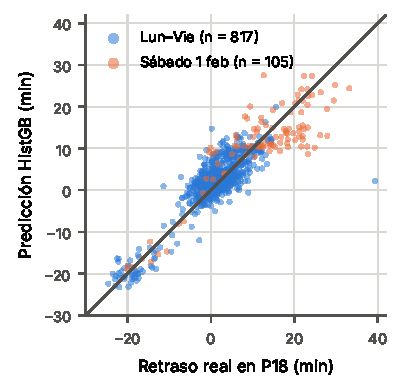
\includegraphics[width=0.85\columnwidth]{figuras/prueba_real_vs_pred.pdf}
\caption{Retraso real y predicho por HistGradientBoosting en P18 (prueba, 922 vueltas). La diagonal marca la predicción perfecta. El sábado se resalta.}
\label{fig:pred}
\end{figure}

\begin{table}[h]
\centering
\caption{MAE (min) por día de prueba}
\label{tab:dia}
\footnotesize
\begin{tabular}{@{}lcccc@{}}
\toprule
\textbf{Día} & \textbf{Vueltas} & \textbf{Persistencia} & \textbf{RF} & \textbf{HistGB}\\
\midrule
Lun 27 ene & 164 & 3,98 & 2,97 & 3,14\\
Mar 28 ene & 149 & 3,20 & 2,36 & 2,10\\
Mié 29 ene & 163 & 3,25 & 2,54 & 2,40\\
Jue 30 ene & 174 & 3,30 & 2,46 & 2,13\\
Vie 31 ene & 167 & 4,07 & 3,07 & 2,88\\
Sáb 1 feb & 105 & 10,16 & 5,19 & 4,61\\
\bottomrule
\end{tabular}
\end{table}

\subsection{Error según el punto de partida (validación cruzada)}\label{sec:curva}
Se repitió la validación cruzada para cada punto de partida $k=5,\dots,17$, con los mismos 5 pliegues y los hiperparámetros elegidos para $k=10$; la prueba no se usó (Fig.~\ref{fig:curva}).
\begin{itemize}
    \item HistGradientBoosting tiene el menor MAE hasta P15. Su ventaja sobre la persistencia es mayor al inicio de la ruta (3,51 frente a 6,82 min en P5) y desaparece al final (1,56 frente a 1,65 min en P16).
    \item La mejora es gradual hasta P12 (MAE de 3,16 min) y se acelera entre P12 y P14 (2,65 min), justo donde el EDA muestra el salto del retraso.
    \item \emph{La meta $R^2\ge0{,}80$ se alcanza desde P14} ($R^2=0{,}81\pm0{,}04$); desde P10 el modelo se queda en $0{,}71\pm0{,}05$.
    \item En P16--P17, Ridge supera ligeramente a HistGradientBoosting (MAE 1,48 frente a 1,56 en P16). Cerca del final, el retraso restante es casi lineal en el último retraso observado, y los hiperparámetros de HistGB se eligieron para $k=10$.
\end{itemize}

\begin{figure*}[t]
\centering
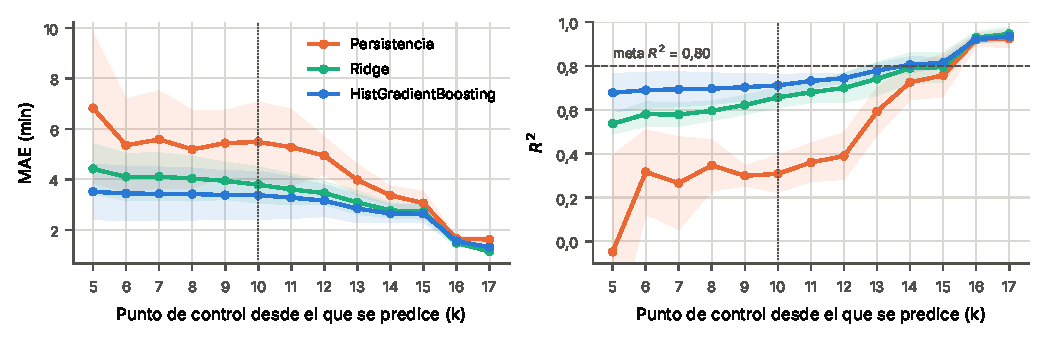
\includegraphics[width=\textwidth]{figuras/curva_por_k.pdf}
\caption{MAE y $R^2$ en validación cruzada según el punto de control desde el que se predice el retraso en P18 (media de 5 pliegues; banda: $\pm1$ desviación estándar). La línea vertical marca el experimento principal ($k=10$).}
\label{fig:curva}
\end{figure*}

\subsection{Sensibilidad del umbral de limpieza}\label{sec:umbral}
Bajar el umbral de ``paso con hora incompatible'' de 60 a 30 min marca 249 pasos en lugar de 156 y deja 3\,066 vueltas de desarrollo en lugar de 3\,082. Comparado sobre las mismas vueltas de validación, el MAE de HistGB en validación cruzada pasa de 3,21 a 3,20 min. La diferencia es muy inferior a la desviación entre pliegues (0,79 min), por lo que el resultado no depende de este umbral y se mantiene el de 60 min.

\subsection{Importancia de las variables}\label{sec:imp}
La importancia por permutación se mide como el aumento del MAE en los pliegues de validación al desordenar cada variable (10 repeticiones). Se muestra en la Fig.~\ref{fig:imp}.
\begin{itemize}
    \item La hora de salida es la variable más importante: 1,33 min su componente seno y 0,58 su componente coseno.
    \item Le sigue el día de la semana (0,74 min), aunque con una variabilidad muy alta entre pliegues. Su importancia es de 1,04 y 2,29 min en los dos pliegues que validan un sábado (18 y 25 ene), y de 0 a 0,33 en los demás.
    \item Entre los retrasos observados, el de P10 es el que más aporta (0,32 min).
    \item La plantilla casi no aporta (0,004 min): su información ya está contenida en la hora de salida.
\end{itemize}

\begin{figure}[t]
\centering
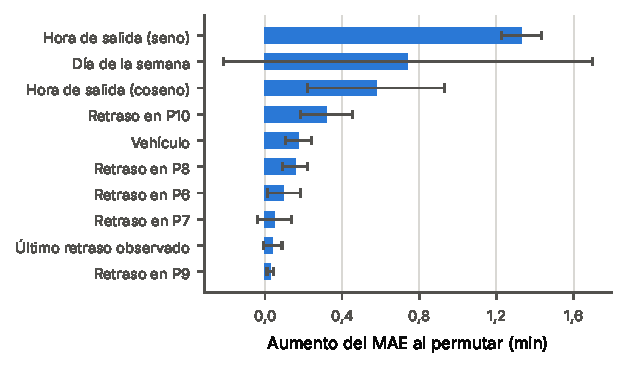
\includegraphics[width=\columnwidth]{figuras/importancia.pdf}
\caption{Importancia por permutación de HistGradientBoosting ($k=10$): aumento medio del MAE en los 5 pliegues de validación; barras de error: $\pm1$ desviación estándar entre pliegues. Se muestran las 10 variables más importantes.}
\label{fig:imp}
\end{figure}

% ═══════════════════════════════════════════════════════════════════════════════
\section{Discusión}

\textbf{Por qué ganan los ensambles.} La persistencia supone que el retraso de P10 se mantiene, pero en estos datos el retraso cambia en la segunda mitad de la ruta según la hora, la plantilla y el día. Los ensambles capturan esas interacciones. La ganancia frente a Ridge (3,41 $\to$ 2,77 min) indica que la relación no es lineal. Esto coincide con \cite{martyanov2026}, que también encuentra que los ensambles de árboles son la mejor opción.

\textbf{Dónde falla el modelo: los sábados.} El análisis de residuos de la prueba muestra que el error se concentra el sábado 1 de febrero. Ese día el retraso mediano en P18 fue de 14,2 min, frente a 0,6--1,6 min de lunes a viernes. Además, el retraso crece de forma brusca entre P10 y P14: la media pasa de 3,6 a 14,7 min. Entre las 9 y las 14 h, el modelo predice 11--13 min cuando el retraso real medio fue de 14--21 min. Los sábados del desarrollo (11, 18 y 25 de enero) muestran la misma tendencia creciente, con medianas de 8,8, 9,5 y 14,2 min. El modelo vio solo tres sábados, de modo que el día de la semana es la variable con menos ejemplos por categoría. Una hipótesis plausible es la congestión de fin de semana en la segunda mitad de la ruta. Las velocidades GPS por tramo permitirían comprobarla. Para mitigarlo, hay tres opciones: más semanas de datos, variables que crucen el sábado con la hora, o un modelo específico para fin de semana. Con solo tres sábados de desarrollo, la última opción no es viable todavía.

\textbf{Un horario nuevo en la prueba.} La plantilla de 168 min reemplaza a la de 170 min justo al empezar la prueba, de modo que la prueba no es solo un periodo posterior: contiene una condición que el modelo no vio. El error en esas vueltas es mayor (3,37 frente a 2,64 min), pero el modelo no colapsa. Una razón es que la hora de salida, la variable más importante, sí está representada; la plantilla en sí casi no aporta. Si los horarios cambian con frecuencia, conviene describir el horario por la franja y el tiempo programado de cada tramo, y no por la duración total.

\textbf{La métrica operativa sigue baja.} Solo el 49\,\% de las predicciones tiene un error de 2 min o menos. El modelo reduce sobre todo los errores grandes (el RMSE baja de 6,15 a 4,04 min), y lo hace más que los pequeños. Desde P10, con 8 puntos de control todavía por recorrer, acertar con un margen de $\pm2$ min sigue siendo difícil.

\textbf{Comparación con el E1.} En el E1, el Random Forest sin ajuste obtuvo un MAE de 2,85 min con el retraso truncado. Ahora HistGB obtiene 2,77 min con el retraso en segundos, el ajuste de hiperparámetros y las nuevas variables. Las cifras no son estrictamente comparables, porque el objetivo cambió de resolución.

\textbf{¿Cuánto $R^2$ es alcanzable desde P10?} La curva por punto de partida (Fig.~\ref{fig:curva}) sugiere que el límite está en la información disponible y no en el modelo. Desde P10, Ridge, Random Forest y HistGB quedan entre 0,66 y 0,71 de $R^2$. El $R^2$ sube rápido solo cuando el bus ya pasó el tramo P12--P14, donde se produce la mayor parte del retraso. Lo que ocurre en ese tramo todavía no se observa en P10, y con estos datos solo puede anticiparse por la hora y el día. Las velocidades GPS de los tramos ya recorridos y del bus precedente son la vía natural para reducir esa incertidumbre.

\textbf{El objetivo depende del horario.} El retraso se mide respecto a un horario que no siempre es realista: la plantilla de 147 min, por ejemplo, termina sistemáticamente adelantada. Por eso, el modelo aprende en parte a corregir el horario. Esto tiene dos consecuencias. Si el operador cambia el horario, como ocurrió al inicio de la prueba, el modelo debe reentrenarse o describir el horario por tramos. Además, parte de la ``predictibilidad'' medida (la hora de salida es la variable más importante) proviene de errores sistemáticos del horario y no de la dinámica del tráfico.

\textbf{Comparación con la literatura.} Martyanov et al.~\cite{martyanov2026} reportan MAE $\approx$ 3,6 min y $R^2\approx$ 0,44, y Petersen et al.~\cite{petersen2019}, 1,99 min. Nuestras cifras (2,77 min; 0,76) no son directamente comparables. Allí se predice para toda una red o una línea y en todas las paradas; aquí, una sola ruta circular, un solo punto objetivo y un horizonte fijo de 8 puntos de control. Además, nuestro $R^2$ se apoya en diferencias grandes y predecibles entre franjas horarias y plantillas. Lo comparable es la conclusión cualitativa: los ensambles de árboles superan a la persistencia y a los modelos lineales, y la hora y la posición en la ruta dominan.

\textbf{Uso operativo.} Con un MAE de 2,77 min, el modelo sirve para anticipar retrasos grandes, del orden de 5 min o más, con 8 puntos de antelación, pero no para avisos al minuto (solo el 49\,\% de las predicciones tiene un error de 2 min o menos). Traducir la predicción a una decisión del despachador, como clasificar la vuelta en adelantada, puntual o retrasada, queda para la entrega final.

\textbf{Limitaciones y validez externa.}
\begin{itemize}
    \item Hay una sola ruta y 27 días: no se capturan la estacionalidad ni otras rutas.
    \item La prueba tiene 6 días y un solo sábado, por lo que los IC son aproximados y el resultado de los sábados descansa en un único día.
    \item El periodo de prueba ya se había usado en el E1 (Sección~\ref{sec:cambios}).
    \item El horario de la tarde cambió al inicio de la prueba (plantilla de 168 min no vista en el desarrollo).
    \item La curva por punto de partida reutiliza los hiperparámetros de $k=10$, lo que puede desfavorecer a HistGB cerca del final de la ruta.
    \item \emph{Sesgo de selección:} el 11\,\% de las vueltas de desarrollo no tiene P18 y se excluye. Esas vueltas salen más tarde (hora media 13,8 frente a 11,2) y son algo más frecuentes en sábado (18\,\% frente a 15\,\%), pero sus retrasos ya observados son similares: mediana de 3,8 frente a 3,7 min en P14 y p75 de 8,7 frente a 7,6 min en P16. El error podría estar ligeramente subestimado en las franjas más congestionadas.
    \item No se usa el GPS.
\end{itemize}

% ═══════════════════════════════════════════════════════════════════════════════
\section{Conclusiones y Trabajo Futuro}

Con solo los datos de control de horarios, un HistGradientBoosting ajustado con validación temporal predice el retraso en el último punto de control desde la mitad de la ruta con un MAE de 2,77 min. Es un 36\,\% menos que la persistencia, y HistGB es mejor en los 6 días de prueba. Frente a Random Forest, la ventaja es pequeña (0,20 min) y no concluyente. Desde P10 no se demostró la meta de $R^2\ge0{,}80$ (0,76 en la prueba y 0,71 en la validación cruzada); en validación cruzada se alcanza desde P14. Los principales obstáculos son los sábados, con un retraso que crece bruscamente en la segunda mitad de la ruta, y un horario de tarde que solo aparece en la prueba. La hora de salida es la variable más importante, y el resultado no depende del umbral de limpieza. La revisión de calidad descartó que los pasos anómalos sean cruces de medianoche y mostró que explican todos los tramos con tiempo negativo.

\textbf{Trabajo futuro (entrega final):}
\begin{itemize}
    \item Variables GPS por tramo, sobre todo para explicar los sábados.
    \item Ajustar hiperparámetros por punto de partida y describir el horario por tramos.
    \item Clasificación de puntualidad y agrupamiento de perfiles de retraso.
    \item Demo interactiva sobre el mapa de la ruta.
\end{itemize}

% ═══════════════════════════════════════════════════════════════════════════════
\section{Entorno Computacional y Reproducibilidad}
\begin{itemize}
    \item \emph{Entorno:} Python 3.13 con numpy 2.5.3, pandas 3.0.5, scikit-learn 1.9.1 y scipy 1.18.1 (versiones fijadas en \texttt{requirements.txt}). Linux, CPU Intel Xeon de 2,1 GHz con 4 núcleos y 15 GB de RAM. El ajuste (\texttt{04}) tarda unos 4 min y los análisis complementarios (\texttt{05}), unos 35 s. Entrenar el HistGB final con las 3\,082 vueltas de desarrollo toma 0,4 s, y predecir una vuelta, menos de 0,01 ms: el costo de cómputo no es una restricción para el uso operativo.
    \item \emph{Aleatoriedad:} semilla 42 en la búsqueda aleatoria, los modelos y el \textit{bootstrap}. Con otras semillas (0, 1 y 2), el mejor MAE de validación cruzada de la búsqueda de HistGB varía entre 3,375 y 3,386 min, y el de Random Forest, entre 3,526 y 3,553 min: las conclusiones no dependen de la semilla.
    \item \emph{Ejecución:} en orden, los scripts \texttt{01}, \texttt{02}, \texttt{04} (con \texttt{-{}-evaluar-prueba} para la evaluación final), \texttt{05} y \texttt{06} de la carpeta \texttt{src/}; instrucciones en \texttt{README.md}.
    \item \emph{Salidas:} todas las tablas de este documento se generan en \texttt{resultados/} y las figuras en \texttt{figuras/}. El archivo \texttt{resultados/PRUEBA\_EVALUADA.txt} registra cuándo se evaluó la prueba y con qué \textit{commit} (\texttt{6445b10}, protocolo congelado).
    \item \emph{Código:} \url{https://github.com/jeremygiraldo/1inf02-machine-learning-project}, rama \texttt{claudia-E2}.
\end{itemize}
\bibliographystyle{IEEEtran}
\begin{thebibliography}{99}

\bibitem{reich2019}
T.~Reich, M.~Budka, D.~Robbins, and D.~Hulbert,
``Survey of ETA prediction methods in public transport networks,''
arXiv:1904.05037, 2019.

\bibitem{kumar2025review}
B.~A. Kumar, R.~Singh, H.~E. Shaji, and L.~Vanajakshi,
``Bus arrival time prediction: A comprehensive review,''
\textit{IEEE Trans. Intell. Transp. Syst.}, vol.~26, no.~6, 2025.

\bibitem{chien2002}
S.~I.-J. Chien, Y.~Ding, and C.~Wei,
``Dynamic bus arrival time prediction with artificial neural networks,''
\textit{J. Transp. Eng.}, vol.~128, no.~5, pp. 429--438, 2002.

\bibitem{jeong2004}
R.~Jeong and L.~R. Rilett,
``Bus arrival time prediction using artificial neural network model,''
in \textit{Proc. 7th IEEE Int. Conf. Intell. Transp. Syst.}, 2004, pp. 988--993.

\bibitem{yu2006}
B.~Yu, Z.~Yang, and B.~Yao,
``Bus arrival time prediction using support vector machines,''
\textit{J. Intell. Transp. Syst.}, vol.~10, no.~4, pp. 151--158, 2006,
doi: 10.1080/15472450600981009.

\bibitem{yu2011}
B.~Yu, W.~H.~K. Lam, and M.~L. Tam,
``Bus arrival time prediction at bus stop with multiple routes,''
\textit{Transp. Res. Part C Emerg. Technol.}, vol.~19, no.~6, pp. 1157--1170, 2011.

\bibitem{achar2020}
A.~Achar, D.~Bharathi, B.~A. Kumar, and L.~Vanajakshi,
``Bus arrival time prediction: A spatial Kalman filter approach,''
\textit{IEEE Trans. Intell. Transp. Syst.}, vol.~21, no.~3, pp. 1298--1307, 2020.

\bibitem{petersen2019}
N.~C. Petersen, F.~Rodrigues, and F.~C. Pereira,
``Multi-output bus travel time prediction with convolutional LSTM neural network,''
\textit{Expert Syst. Appl.}, vol.~120, pp. 426--435, 2019.

\bibitem{martyanov2026}
V.~Martyanov, A.~Budzy{\'n}ski, A.~Czerepicki, and M.~Koz{\l}owski,
``Interpretable machine learning for identifying the determinants of bus delays,''
\textit{Arch. Transp.}, vol.~77, no.~1, pp. 7--26, 2026,
doi: 10.61089/aot2026.mnrkh112.

\bibitem{boudabbous2026}
E.~Boudabbous, M.~Karaa, L.~Sboui, J.~Montecinos, and O.~Alam,
``Scalable transit delay prediction at city scale: A systematic approach with multi-resolution feature engineering and deep learning,''
\textit{J. Syst. Archit.}, vol.~176, 2026; preprint arXiv:2601.18521.

\bibitem{degeler2021}
V.~Degeler, L.~Heydenrijk-Ottens, D.~Luo \textit{et al.},
``Unsupervised approach towards analysing the public transport bunching swings formation phenomenon,''
\textit{Public Transport}, vol.~13, pp. 533--555, 2021,
doi: 10.1007/s12469-020-00251-z.

\bibitem{rojas2023}
L.~Rojas-Bustamante, C.~Alfaro, I.~Molero, D.~Aparicio, and M.~Nunez-del-Prado,
``Profiling public service accessibility based on the public transport infrastructure,''
in \textit{Information Management and Big Data (SIMBig 2022)}, CCIS vol.~1837, Springer, 2023,
doi: 10.1007/978-3-031-35445-8\_14.

\bibitem{cusco2024}
E.~F. Carcausto-Mamani, E.~R. Rojas-Cahuana, E.~Alvarez-Mamani, and H.~Vera-Olivera,
``Multivariable-unistep prediction of travel times in public transport buses using LSTM and convolutional LSTM,''
in \textit{Information Management and Big Data (SIMBig 2023)}, J.~A. Lossio-Ventura \textit{et al.}, Eds., CCIS vol.~2142.
Cham, Switzerland: Springer, 2024,
doi: 10.1007/978-3-031-63616-5\_4.

\bibitem{traverso2025}
D.~Traverso, G.~Pacheco, and P.~Casta{\~n}eda,
``T-RAPPI: A machine learning model for the Corredor Metropolitano,''
in \textit{Proc. 11th Int. Conf. Vehicle Technol. Intell. Transp. Syst. (VEHITS)}, 2025, pp. 374--381,
doi: 10.5220/0013220700003941.

\bibitem{wang2018wdr}
Z.~Wang, K.~Fu, and J.~Ye,
``Learning to estimate the travel time,''
in \textit{Proc. 24th ACM SIGKDD Int. Conf. Knowl. Discov. Data Min.}, 2018, pp. 858--866.

\bibitem{hu2022deepreta}
X.~Hu \textit{et al.},
``DeeprETA: An ETA post-processing system at scale,''
arXiv:2206.02127, 2022.

\bibitem{li2024arrivalnet}
Z.~Li, P.~Wolf, and M.~Wang,
``ArrivalNet: Predicting city-wide bus/tram arrival time with two-dimensional temporal variation modeling,''
arXiv:2410.14742, 2024.

\bibitem{tcrp2003}
Transportation Research Board,
\textit{Transit Capacity and Quality of Service Manual}, 2nd ed., TCRP Report 100.
Washington, DC, USA: TRB, 2003.

\bibitem{bergmeir2012}
C.~Bergmeir and J.~M. Ben{\'i}tez,
``On the use of cross-validation for time series predictor evaluation,''
\textit{Inf. Sci.}, vol.~191, pp. 192--213, 2012.

\bibitem{kaufman2012}
S.~Kaufman, S.~Rosset, C.~Perlich, and O.~Stitelman,
``Leakage in data mining: Formulation, detection, and avoidance,''
\textit{ACM Trans. Knowl. Discov. Data}, vol.~6, no.~4, pp. 1--21, 2012.

\bibitem{grinsztajn2022}
L.~Grinsztajn, E.~Oyallon, and G.~Varoquaux,
``Why do tree-based models still outperform deep learning on typical tabular data?''
in \textit{Adv. Neural Inf. Process. Syst. (NeurIPS)}, 2022.

\bibitem{breiman2001}
L.~Breiman,
``Random forests,''
\textit{Mach. Learn.}, vol.~45, no.~1, pp. 5--32, 2001.

\bibitem{chen2016}
T.~Chen and C.~Guestrin,
``XGBoost: A scalable tree boosting system,''
in \textit{Proc. 22nd ACM SIGKDD Int. Conf. Knowl. Discov. Data Min.}, 2016, pp. 785--794.

\bibitem{ke2017}
G.~Ke \textit{et al.},
``LightGBM: A highly efficient gradient boosting decision tree,''
in \textit{Adv. Neural Inf. Process. Syst.}, vol.~30, 2017.

\bibitem{hochreiter1997}
S.~Hochreiter and J.~Schmidhuber,
``Long short-term memory,''
\textit{Neural Comput.}, vol.~9, no.~8, pp. 1735--1780, 1997.

\bibitem{lundberg2017}
S.~M. Lundberg and S.-I. Lee,
``A unified approach to interpreting model predictions,''
in \textit{Adv. Neural Inf. Process. Syst.}, vol.~30, 2017.

\bibitem{pedregosa2011}
F.~Pedregosa \textit{et al.},
``Scikit-learn: Machine learning in Python,''
\textit{J. Mach. Learn. Res.}, vol.~12, pp. 2825--2830, 2011.

\end{thebibliography}

\end{document}
